\documentclass[12pt,letterpaper]{article}

\usepackage[hmargin=1in,bottom=1in,top=1in]{geometry}
\usepackage[latin1]{inputenc}
\usepackage{amsmath}
\usepackage{amsfonts}
\usepackage{amssymb}
\usepackage{graphicx}
\usepackage{url}
\usepackage[toc,page]{appendix}
\usepackage{setspace}
\usepackage{pdfpages}

\usepackage{ulem}
\normalem

% push footnotes to the bottom of the page unconditionally
\usepackage[bottom]{footmisc}

\usepackage[pdftex]{hyperref}
\hypersetup{
	pdfauthor={Neil Isaac and Keyi Shi},
	pdftitle={Implementation of a virtual FPGA architecture},
	pdfsubject={Virtual FPGA fabrics},
	colorlinks=true,
	anchorcolor=black,
	linkcolor=blue,
	citecolor=blue,
	filecolor=blue,
	pagecolor=blue,
	urlcolor=blue,
	frenchlinks=false,
	pagebackref=true,
	bookmarks=true}

% make links to figures jump to position above the figure
%\usepackage[all]{hypercap}

%\usepackage{titling}
%\usepackage{listings}
%\lstset{language=c}

% fancyhdr - use top=1.5in
%\usepackage{fancyhdr}
%\pagestyle{fancy}
%\fancyhead[L]{\leftmark}
%\fancyhead[R]{\thepage}
%\fancyhead[CF]{}
%\setlength{\headheight}{16pt}

\setlength{\parindent}{0in}
\setlength{\parskip}{1.0 \baselineskip}
\setlength{\footnotesep}{1.0 \baselineskip}
\setlength{\skip\footins}{2.0 \baselineskip}

\bibliographystyle{IEEEtran}

\usepackage{color}
\newcommand{\note}[1]{}
% comment out the next line to hide draft notes
\renewcommand{\note}[1]{\textcolor{red}{[#1]}}
\newcommand{\citationneeded}[0]{\note{citation needed}}

\newenvironment{enumeration}{
	\setlength{\topsep}{0.0pt}
	\setlength{\partopsep}{0pt}
	\setlength{\parskip}{0pt}
	\setlength{\parsep}{0pt}
	\begin{enumerate}
		\setlength{\itemsep}{0pt}}
	{\end{enumerate}}

\newenvironment{itemlist}{
	\setlength{\topsep}{0pt}
	\setlength{\partopsep}{0pt}
	\setlength{\parskip}{0pt}
	\setlength{\parsep}{0pt}
	\begin{itemize}
		\setlength{\itemsep}{0pt}}
	{\end{itemize}}

\newcommand{\sectref}[1]{Section \ref{#1}}
\newcommand{\figref}[1]{Figure \ref{#1}}
\newcommand{\tableref}[1]{Table \ref{#1}}
\newcommand{\overlay}{Overlay FPGA }

%\renewcommand{\thefootnote}{\roman{footnote}}

\begin{document}

	\begin{titlepage}
\begin{center}


\includegraphics[scale=1.0]{ecelogo.png}

\vspace{1 \baselineskip}

\textsc{
\Large University of Toronto\\
\large Department of Electrical and Computer Engineering \\
\large ECE496 Design Project
}

\vspace{2 \baselineskip}

{\Large \bfseries Virtual FPGA fabrics} \\
{\Large \bfseries Implementation of a Virtual FPGA Architecture}

\vspace{2 \baselineskip}

{\large \bfseries Final Report} \\

\vspace{2 \baselineskip}

{\large March 22, 2012}

\vfill

\begin{tabular*}{4in}{l @{\extracolsep{\fill}} l}
\textbf{Neil Isaac} & \textbf{Keyi Shi} \\
\texttt{n.isaac@utoronto.ca} & \texttt{keyi.shi@utoronto.ca} \\ & \\
\emph{Project ID:} & 2011017 \\
\emph{Supervisor:} & Jason Anderson \\
\emph{Administrator:} & Ross Gillett \\
\emph{Section:} & \#7 \\
\end{tabular*}

\end{center}
\end{titlepage}



	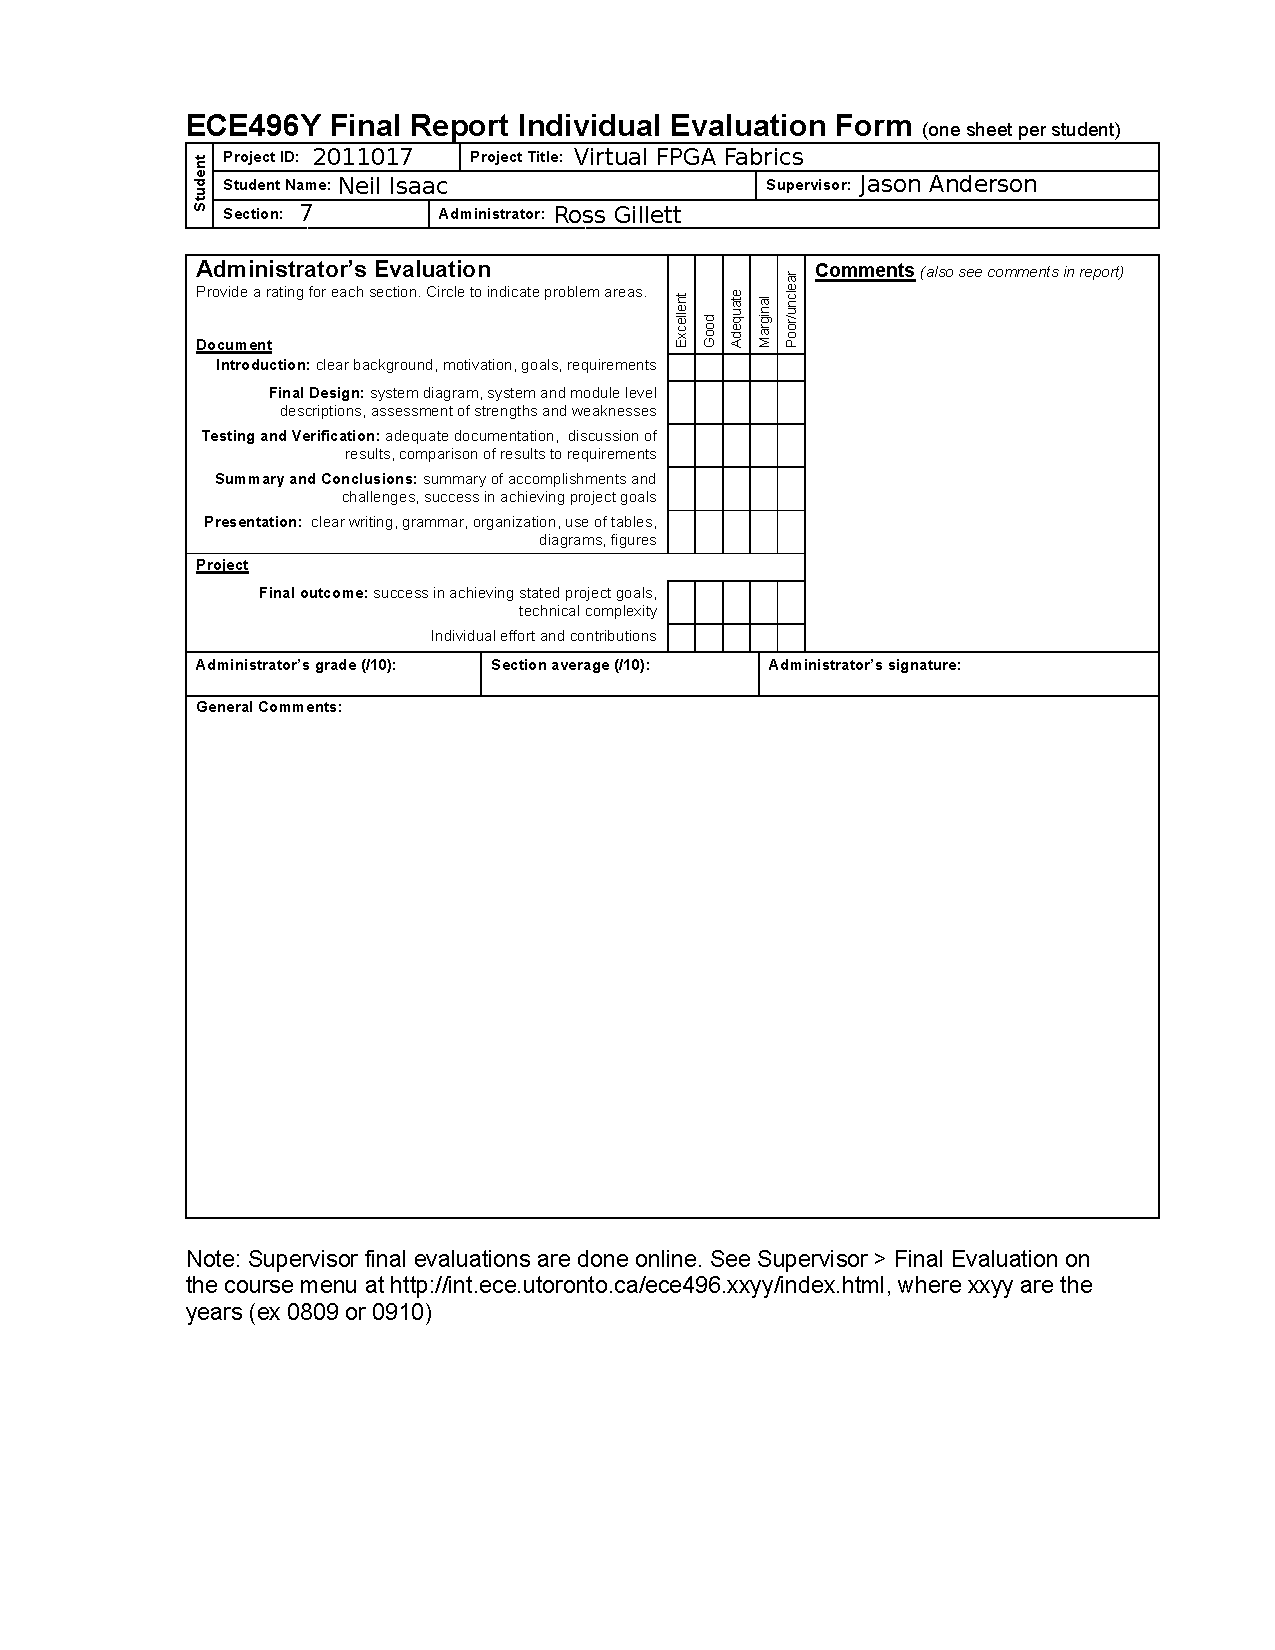
\includepdf{cover-neil.pdf}
	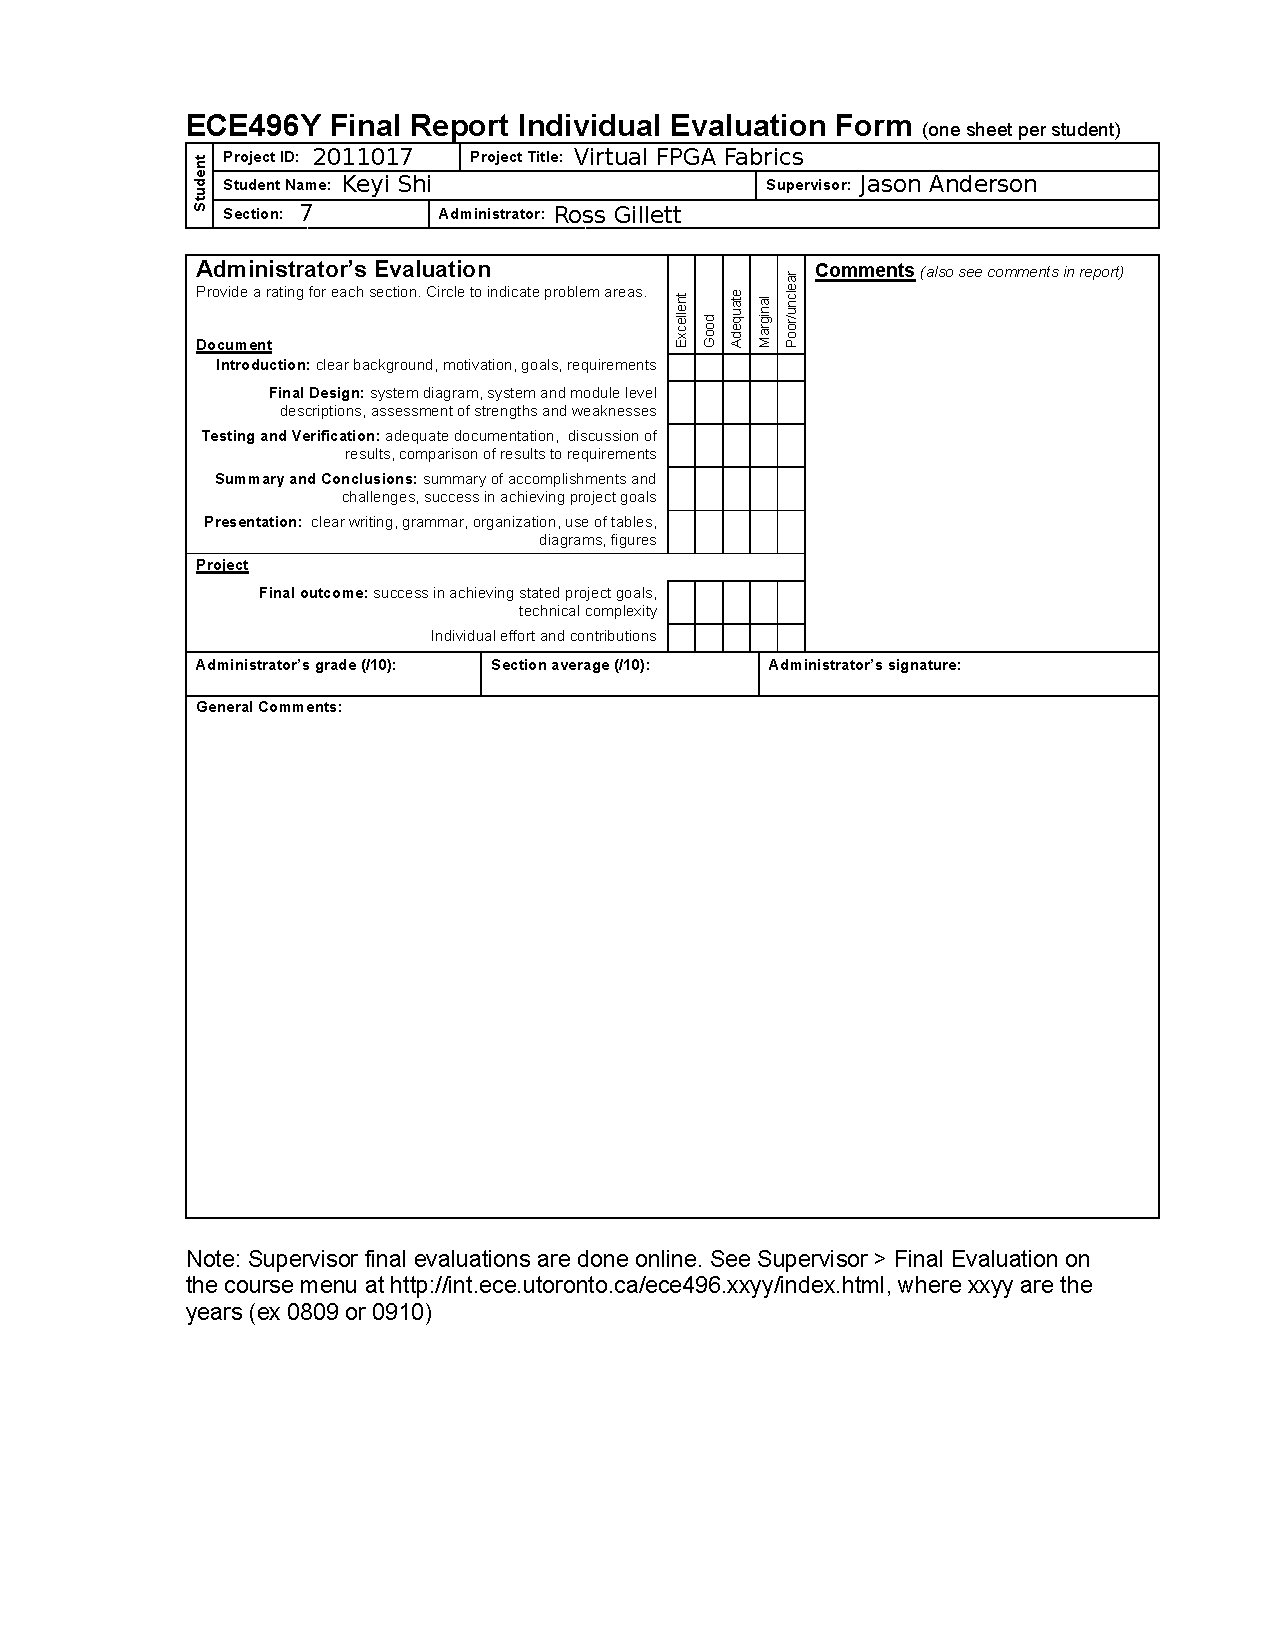
\includepdf{cover-keyi.pdf}

	\section{Attribution Table}

{\footnotesize
\begin{tabular}{|l|l|l|}
	\hline
	\textbf{Section} & \textbf{Neil} & \textbf{Keyi} \\
	\hline \hline
	Executive Summary & ET & RD \\
	\hline
	Background and Motivation & RD & ET \\
	Project Goal & RD & ET \\
	Project Requirements & RD & ET \\
	Validation and Acceptance Tests & MR, ET & RD \\
	\hline
	Design Alternatives & RS, MR & RD \\
	Assessment of Proposed Design & ET & RD \\
	System-level Overview & RD, ET & MR \\
	Module-level Overview & ET & RD \\
	\hline
	Work Breakdown Structure & RD & ET \\
	Gantt Chart & RD & RS, ET \\
	Financial Plan & RD & ET \\
	Feasibility Assessment & ET & RD \\
	\hline
	All & FP, CM & FP \\
	\hline
\end{tabular}
}

\subsection*{Abbreviation Codes}

{\footnotesize
\begin{tabular}[width=7in]{|l|l||l|l|}
	\hline
	RS & research and information & \multicolumn{2}{l|}{``All'' row entries} \\ \hline
	RD & wrote first draft & FP & final read through \\ \hline
	MR & major revision & CM & compiling elements \\ \hline
	ET & editing spelling grammar and expression & OR & other (describe OR1, OR2, etc) \\ \hline
\end{tabular}
}

\subsection*{Signatures}

By signing below, you verify that you have read the attribution table and agree that it accurately reflects your contribution to this document.

\vfill

\hrule
Neil Isaac \hspace{1in} Date \hspace{1in} Keyi Shi \hspace{1in} Date



	\onehalfspace

	\thispagestyle{empty}
\section*{Executive Summary}

% No more than 1 page
% Should show clear understanding of AUDIENCE and PURPOSE
% Readable as a stand-alone document, clearly differentiated from an introduction
% Give the contest and MOST IMPORTANT information in the document in a unified fashion

Academic studies of Field Programmable Gate Array (FPGA) chip architecture rely on simulations, as commercial FPGA chips contain proprietary designs that make their underlying architecture inaccessible to academic researchers.
The goal of this project is to provide a physical platform for researchers to carry out FPGA architecture studies.
The finished design should capable of running common benchmark circuits.

The proposed design is to implement an Overlay FGPA on an existing, commercially available FPGA chip.
Using a commercial FPGA as the physical medium for this project makes the design cheaper and more accessible to researchers, as they may have an appropriate FPGA chip already.


We have selected the Xilinx Virtex 5 FPGA as our development platform because we can use its native logic units directly.
This will limit the models of FPGA chips that the overlay circuit can be implemented on, but it should reduce the design's area overhead and improve its timing characteristics.
The features we will use on the Virtex 5 are forward-compatible with all current-generation Xilinx FPGA products, allowing the researcher to use a variety of FPGAs.

The validation of the design will involve testing a set of benchmark circuits by placing and routing them with VPR, then transferring them to the FPGA overlay.
The circuits can then be tested for correct behavior, confirming that the overlay design can be correctly programmed using VPR output, and that the inputs and outputs to the design are functioning properly.

The current budget for the proposed design is \$14.00 and will be covered by the students.
The required FPGA development boards and software licenses have been provided by the supervisor.

We have designed and tested the modules required to build one tile of the Overlay FGPA.
By December, we expect to have assembled a grid of tiles and have software support for programming the logic cells.



	\pagenumbering{roman}

	\section*{Acknowledgements}

We would like to thank our supervisor, Professor Jason Anderson for providing input and feedback throughout the project.


	\section*{Group Highlights}

In order to build a working \emph{Overlay FPGA}, we produced the following:
\begin{itemize}
\item Verilog for the individual FPGA building-blocks: the logic cell, logic block, connection block, and the switch block. (Keyi)
\item Verilog to connect the building block components together in a grid and feed the programming signals through them. (Keyi)
\item Verilog circuit to interface with the UART to enable serial programming of the Overlay FPGA. (Neil)
\item Scripts to run the third-party tools which will process an input circuit (from the user) and produce a valid placment and routing. Some adjustments need to be made so the tools can read each others' outputs. (Neil)
\item Software to convert the placement and routing into a programmable bitstream. (Neil)
\end{itemize}

Our Overlay FPGA circuit meets the functional requirements and objectives set out in our project proposal.

We found that overhead of implementing and FPGA on an FPGA was higher than we extected because some resources we used extensively were limited.
Due to this limitation, we reduced our target size constraint for the Overlay FPGA from 3000 logic cells down to 100 logic cells. % FIXME: 100?
Although this sounds much lower, it is still large enough to implement working overlay designs.

The size restriction limits the size of circuits our \overlay can support, so we can no longer accommodate the MCNC benchmark circuits we originally planned to use.
We developed our own simple \emph{unit-test} circuits which each test very specific functionality.
These new test circuits allowed us to incrementally track down basic issues with our bitstream.


	
	\pagebreak
	
	\section*{Highlights for Neil Isaac}

My main contributions to the project were:
\begin{itemlist}
	\item components of the \overlay Verilog design,
	\item compiling and scripting the third-party tool flow, and
	\item writing the software to produce and program the bitstream.
\end{itemlist}

The basic components of the \overlay are the \emph{connection block}, \emph{switch block} and the \emph{logic block}.
The logic block consists of a variable number of \emph{logic elements} and flip-flops which are the fundamental pieces that allow a user to implement their circuit on the \overlay.
We designed the basic components so they can be replicated and connected on a grid of arbitrary size, and with an arbitrary amount of routing interconnect resources.
The level of configurability we support limits the scope of optimizations we could consider, so our highly configurable \overlay takes more resources on the physical FPGA than a may be strictly necessary.

The third-party software flow consists of \emph{ODIN} for synthesis, \emph{ABC} for technology mapping, \emph{T-VPack} for clustering, and \emph{VPR 5} for placement and routing.
My work on the tool flow involved figuring out how to use the individual tools, and producing the appropriate formats of files for each stage.
Each of these tools had various bugs or technical issues I needed to work around.

The bitstream generation software I wrote reads the \emph{BLIF} format function tables from ABC, the connectivity netlist from T-VPack, and the placements and routing files from VPR.
I needed to correlate the files to find the location of each functional element in the placement file, its inputs from the netlist file, and how the inputs are connected from the routing file.
In some cases, this data needs to be inferred because the tools don't fully specify the placements or connections.


	\section*{Highlights for Keyi Shi}

My contributions to the final design were:
\begin{itemlist}
	\item shift multiplexing for all logic tile modules
	\item component modules for the overlay verilog design
	\item verilog overlay tile boundary design and optimization
\end{itemlist}

Multiplexers are used extensively in all our verilog modules.
Each module has different multiplexing requirements, and one of our design goals was to have a configurable size/routing parameters; as such, the sizes of multiplexers required by our design vary module to module, parameter to parameter.
I designed a flexible multiplexer capable of changing its size based on the number of inputs required, and this multiplexer is what drives all our overlay modules.

I focused on the routing elements of the overlay design, building the switch block and connection block modules and ensuring their compatibility with each other and the logic block.
The modules were all designed to be flexible, capable of accepting user parameters and changing their sizes and arrangements to fit user needs.
The modules also went through bitstream testing to make sure they behaved correctly under all use cases.

The verilog overlay tile combined basic verilog components into a single module, capable of being replicated in a grid formation to create the final overlay.
The boundaries of the overlay required special modules to tie the grid together and interface between the overlay's internal and input/output signals.
I wrote the boundary modules and debugged/optimized the overlay design, ensuring all signals between tiles are routed correctly, and the boundary signals are gathered into their appropriate input/output pads.
I tested the overlay with manual and generated bitstreams to debug both the overlay hardware and the bitstream software.

	\singlespace

	\setcounter{tocdepth}{1}
	\tableofcontents
	%\listoffigures
	%\listoftables
	
	\pagebreak

	\pagenumbering{arabic}

	\onehalfspace

	\section{Introduction}

This report explains the motivation, implementation and testing, and limitations of our Overlay FPGA circuit.


\subsection{Background and Motivation}

Academic researchers who study Field Programmable Gate Array (FPGA) design commonly use variations of an FPGA design architecture, described by Kuon et al\cite{fpga}, which we will refer to as the \emph{Academic FPGA Model}.
While FPGA chips are available from a variety of commercial vendors, their inner design is proprietary, making their architectures difficult to study.
Furthermore, there is no existing physical implementation\footnote{Alex Brant is also developing a comparable FPGA overlay platform with Prof. Guy Lemieux at University of British Columbia.} of an Academic FPGA Model.

VPR\cite{vpr} is an open-source placement and routing tool used in FPGA architecture research.
It can handle many variations of the Academic FPGA Model.
It is not currently possible to implement circuits produced by VPR on a commercial FPGA.\footnote{A technology-mapped input netlist for VPR can be converted to an Altera Quartus VQM netlist file using \emph{nettovqm}\cite{nettovqm}, but the placement and routing can not be converted.}

Computer Aided Design (CAD) researchers who work on placement and routing algorithms for FPGA designs are presently limited to using simulations to evaluate or verify their work.
They may be interested in testing circuits on a physical medium because it would be much faster than simulating the circuits.



\subsection{Project Goal}

The goal of this project is to design a circuit design based on the Academic FPGA Model.
Researchers will be able to use the circuit to study FPGA architecture and CAD algorithms with circuits produced by VPR.



\subsubsection{Functional Requirements}

An Overlay FGPA circuit that will:

\begin{itemlist}
	\item Work on a commercially available FPGA chip.
	\item Be re-programmable over a serial interface after being flashed to the FPGA.
	\item Have a tunable number and arrangement of logic cells, and have tunable connectivity parameters. 
	\item Support inputs to and outputs from test circuits programmed onto the Overlay FGPA.
\end{itemlist}

A software program that can:
\begin{itemlist}
	\item Translate VPR placement and routing data for a test circuit into a bitstream for the Overlay FGPA.
	\item Program the bitstream onto the Overlay FGPA to implement the circuit.
\end{itemlist}

\subsubsection{Constraints}

\begin{itemlist}
	\item Support 6-input logic elements, which allows for comparison with current generation commercial FPGAs.
	\item Fit at least 100 overlay logic elements on the Virtex 5 FPGA.  This number was chosen to be adequately large for our proof of concent.  100 cells will fit our test circuits fit, and concevable circuits can be implemented by participants at the design fair.
	%\item The overlay circuit must support at least 3000 logic cells\footnote{3000 logic cells was chosen as the minimum target because the largest of the ``Golden 20'' circuits, \emph{``s38417''} requires 2567 6-input logic cells\cite{synthesis-density}.} in order to accommodate the \emph{``Golden 20''} MCNC benchmark circuits\footnote{The ``Golden 20'' MCNC circuits are available in BLIF format at \url{http://www.ece.ubc.ca/~julienl/benchmarks.htm}.} commonly used in FPGA research.
\end{itemlist}


\subsubsection{Objectives}

\begin{itemlist}
	\item Be compatible with a family of commercial FPGAs that are available to researchers.
	\item Use the native logic cells in the physical FPGA directly in the overlay FPGA design to reduce area and latency.
	\item Be fast enough that it outperforms software emulation of most test circuits.
\end{itemlist}


	\section{Final Design}


\subsection{System overview}
\label{system-overview}

\figref{system-diagram} shows the high-level system interactions of the components used in our project.
The components we built are shown in solid rectangles.

The finished project consists of three main parts: The overlay FPGA, bitstream generation software, and interfacing of inputs/outputs of the overlay FPGA.

The \emph{Overlay FPGA} is a Verilog HDL circuit implementation of the Academic FPGA model which is constructed as an overlay on a Xilinx FPGA board.
The arrangement, size and connectivity of the overlay circuit is controllable via parameters in the source Verilog.
The overlay FPGA consists of organized tiles of \emph{logic block}, \emph{connection block}, and \emph{switch block} modules.
Together, these modules allow the overlay FPGA to implement different logic circuits.

\begin{figure}[!h]
	\centering
	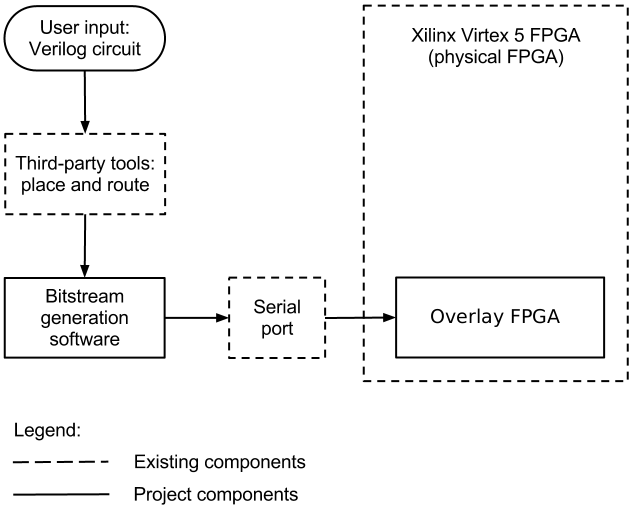
\includegraphics[scale=0.6]{system.png}
	\caption{System overview}
	\label{system-diagram}
\end{figure}

The \overlay can be configured to implement user-specified \emph{test circuits} that have been placed and routed by VPR.
This is achieved using the \emph{bitstream generation and programming software} that translates the VPR output circuit into a bitstream that the overlay FPGA understands.
The bitstream is then injected into the overlay FPGA via a \emph{serial interface}.
The FPGA receives and decode the bitstream into the appropriate test circuits on the overlay.

Finally, the circuits on the overlay FPGA are controlled by connecting devices such as switches and LEDs connected through the physical FPGA.



\subsection{Module design}

The \emph{Overlay FPGA} is composed of a two-dimensional array of \emph{Logic tiles}.
The logic tiles make it easier to build a large overlay, and help keep the internal 
logic modules organized.
Each logic tile consists of one \emph{logic block module}, two \emph{connection block modules}, 
and one \emph{switch block module}.
\figref{tile-diagram} shows the internal composition of a single logic tile.

\begin{figure}[!h]
	\centering
	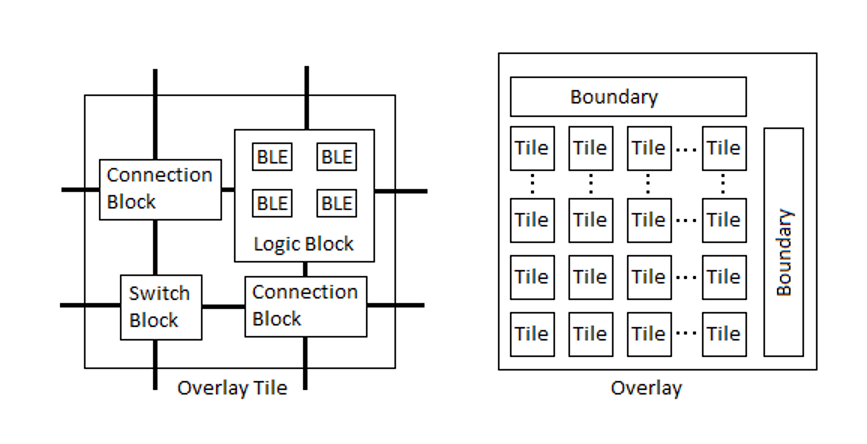
\includegraphics[scale=0.7]{overlay.png}
	\caption{Logic tile and tile arrangement}
	\label{tile-diagram}
\end{figure}

The \emph{Logic block module} consists of programmable look-up tables that perform all of the logical 
funcionality required by the circuit.
A logic block module may be composed of multiple look-up tables, the number of which 
can be determined by verilog parameters.

The \emph{Connection block} and \emph{Switch block} modules regulate the routing of signals in the overlay.
\emph{Connection blocks} connect logic block signals to buses that run throughout the 
overlay.
\emph{Switch blocks} control the routing between buses when they cross each other.

\begin{figure}[!h]
	\centering
	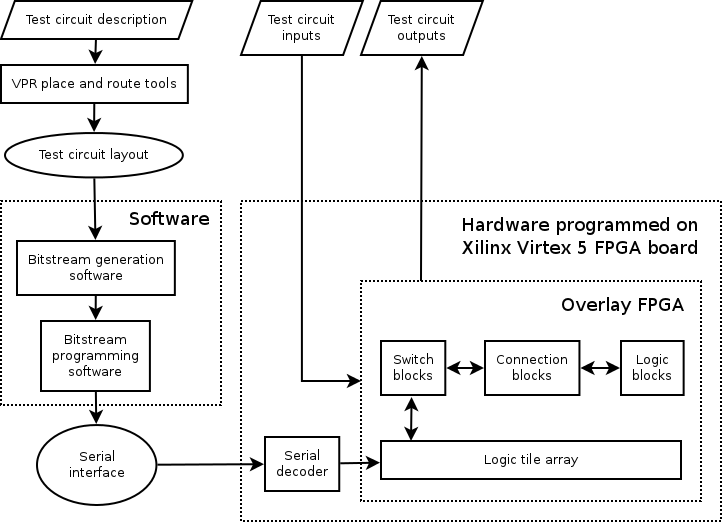
\includegraphics[scale=0.6]{modules.png}
	\caption{Module overview}
	\label{module-diagram}
\end{figure}

\figref{module-diagram} shows the relationship between the higher-level modules.

The \emph{Bitstream generation software} is a program that translates VPR output circuits into a bitstream capable of programming the overlay FPGA directly.
The program consists of functions that parse the output from VPR and generate the 
appropriate bitstream from the parsed information.

The \emph{Bitstream programming software} takes the bitstream formed by the bitstream generator and formats it for proper transmission over a serial interface.

The \emph{Serial decoder} is a circuit attached to the overlay FPGA that receives the 
bitstream sent through the serial interface.
It decodes and extracts the bitstream from the serial format, then injects it into the overlay circuit to configure the overlay.



\subsection{Assessment of design}

The decision to take advantage of the custom 32-bit shift registers in implementing our design entails the following trade-offs versus using only basic Verilog logic:
\begin{itemlist}
	\item The design is more efficient area and timing-wise.
	\item The data describing the circuit (known as the \emph{bitstream}) which is needed to program the design will be larger.
	\item The maximum size of the design will be limited by the amount of 32-bit shift registers available on the FPGA board, as opposed to the amount of flops.
	\item The design will be incompatible with boards that do not have custom 32-bit shift registers
\end{itemlist}

We have decided that performance efficiency outweighs the negative aspects of the larger bitstream and limitation of implementation platforms.
If the design is successful, adaptations can be made in the future to support the implementation of the design on more FPGA boards.

We have also looked into using a Clos network for the logic block crossbar.
Currently, the crossbar is implemented using layered multiplexers built from 32-bit shift registers for each lookup table input, and is the most resource-heavy part of the tile.
By replacing all the input multiplexers with a large Clos network, it is possible to reduce the number of shift registers consumed by up to 35\%.
However, the fact that we only have 32-bit shift registers available as building blocks severely restricts the size of the crossbar, and would have removed the flexibility of choosing the number of logic block inputs currently built into the design.
Additionally, the algorithm for routing the Clos network is much more complex than the current crossbar design; the signal path to each lookup table input are dependent on each other, and cannot be routed individually.
There are existing algorithms for routing Clos networks, but they focus on networks where one input can only route to one output.
For our design, we need a network that can route multiple outputs from a single input.
We were unable to develop our own algorithm for the Clos network due to time constraints.
Because of these reasons, we decided against incorporating Clos networks into our current design.
For future improvements, we may return to Clos networks.



	\section{Testing and Verification}

We performed 4 tests on our final design, 1 test to ensure our hardware works correctly, 1 test to verify our software, and 2 tests on the full work flow to confirm that the project is working as a whole.

\subsection{Hardware Test}

To test that our overlay tiles are working correctly, we built a single tile onto the Virtex 5 FPGA and connected the inputs and outputs of the tile to the switches and LEDs of the FPGA.
We then pushed in a manually composed bitstream through a serial connection to program the tile's function and routing.
Once the tile was programmed, we verified the behaviour of the tile against what we expected from the bitstream, including the functions in the lookup tables, and the routing of input and output signals.
The tile can be re-programmed as many times as we like to test different functions and signal routing.

Excerpt from our manually generated bitstream:
0FFFFFFFFFFFFFFFE
18000000000000000
0FFFFFFFFFFFFFFFF
08888888888888888

The above snippet programs the four 6-input lookup tables and their connected flops.
The leftmost value indicates whether or not the output of the lookup table is routed through a flop (0=no, 1=yes), and the rest determines the function of the lookup table itself.
From the top, the lookup tables are programmed as follows: 6-input OR gate, 6-input AND gate with flop, always 1, 2-input AND gate.

The test showed that our tile was fully functional, behaving as expected in both lookup table functionality and correct routing.
The test proved that our project satisfied the following requirements:
\begin{itemlist}
	\item H1: The tile was implemented on a Virtex 5 FPGA chip
	\item H3: The tile only needed to be built once on the chip, after which it was re-programmable via serial cable without the need to be re-flashed onto the chip.
	\item H4: The tile had connectivity to the switches and LEDs of the chip
	\item S2: Our bitstream sending/receiving software operated correctly in order to program the tile
	\item G1: The tile implemented four 6-input lookup tables
\end{itemlist}

\subsection{Software Test}

To test our bitstream generation software, we wrote simple circuits in verilog, then used our selected third-party software to synthesize, place and route the circuits according to our architecture.
We then took the resultant output and used our software to generate a bitstream capable of programming our overlay circuit.
We went through the generated bitstream manually to ensure the logic and routing matched the overlay, and that it was of the appropriate format for the overlay.
Because of the size of the bitstream, this test is restricted to simple circuits on a small overlay.

The bitstream passed manual inspection; it was structured correctly and the logic and routing matched the third-party software outputs.
The test proved that our project satisfied the following requirements:
\begin{itemlist}
	\item S1: The software was successful in translating VPR placement and route data into a bitstream appropriate for the overlay FPGA
\end{itemlist}

\subsection{Full Tool Flow Test}

Finally, to test the project as a whole, we combined the hardware and software tests, building test circuits in verilog, passing them through VPR and translating the output into a bitstream, and injecting the bitstream onto a full overlay on the Virtex 5 for testing.

We first tested the project with a simple buffer circuit, where inputs to the overlay were connected directly to outputs.
When the buffer proved successful, we moved on to a slightly more complex circuit, an 8-bit adder.

Verilog code for the adder:

\begin{tabular}{|p{7cm}|}
\hline
\begin{verbatim}
module test( in, out);

input  [7:0] in;
output [7:0] out;

assign out = in[7:4] + in[3:0];

endmodule
\end{verbatim}
\\ \hline
\end{tabular}

% for each requirement #, report final result. comment on degree of compliance.
% can add more detailed comments after the table.

% refer to appendix b

% show evidence (vpr screenshots, etc)


	\section{Summary} % and Conclusions

Overall, the project succeeded in what we set out to do.
We met all of our final goals and requirements, producing a flexible overlay FPGA design and tool flow that is capable of implementing a user-specified verilog circuit on the overlay.
We were able to produce a functioning buffer and adder on an 8x8 overlay using our custom tool flow, demonstrating the functionality of all parts of our project (overlay circuit, bitstream generation, bitstream injection).

We believe that our design idea has the potential to become a useful tool for FPGA researchers to test custom architectures or CAD algorithms on real hardware.
The current design is a successful proof-of-concept; it may be useful to some researchers, but others may require a lower overhead.
Some overhead reduction can be achieved by optimizing the structure of the \overlay, by using Clos networks for example.

Modern FPGAs include a lot of fixed-function blocks (\emph{hard macros}) that implement common functions such as multipliers and memories in order to reduce the overhead of using an FPGA for circuits containing many instances of these elements.
A possible extension to our project would be to encorporate \emph{hard macros} available on the Virtex 5 in our overlay circuit.

With our \overlay design, a researcher could easily instantiate the overlay in an FPGA-based embedded system with a \emph{soft microprocessor} such as Xilinx's MicroBlaze.
This would enable research on using re-programmable hardware in embedded systems.

% Did you meet your project goals and requirements, as demonstrated through your validation and acceptance tests?
% To what extent does your testing and verification work prove out your final design?
%  Were your design ideas proven out? If not, explain why.
% What are the key conclusions to be drawn from your project?
% Where is the kind of work you did in your project used or potentially useful in state-of-the-art, industry, academe, or society?




	\pagebreak
	%\nocite{*} % show uncited entries in the bibliography
	\bibliography{ref}
	\addcontentsline{toc}{section}{References}

	\pagebreak

	\begin{appendices}
		\section{Gantt Chart}
\label{gantt-chart}

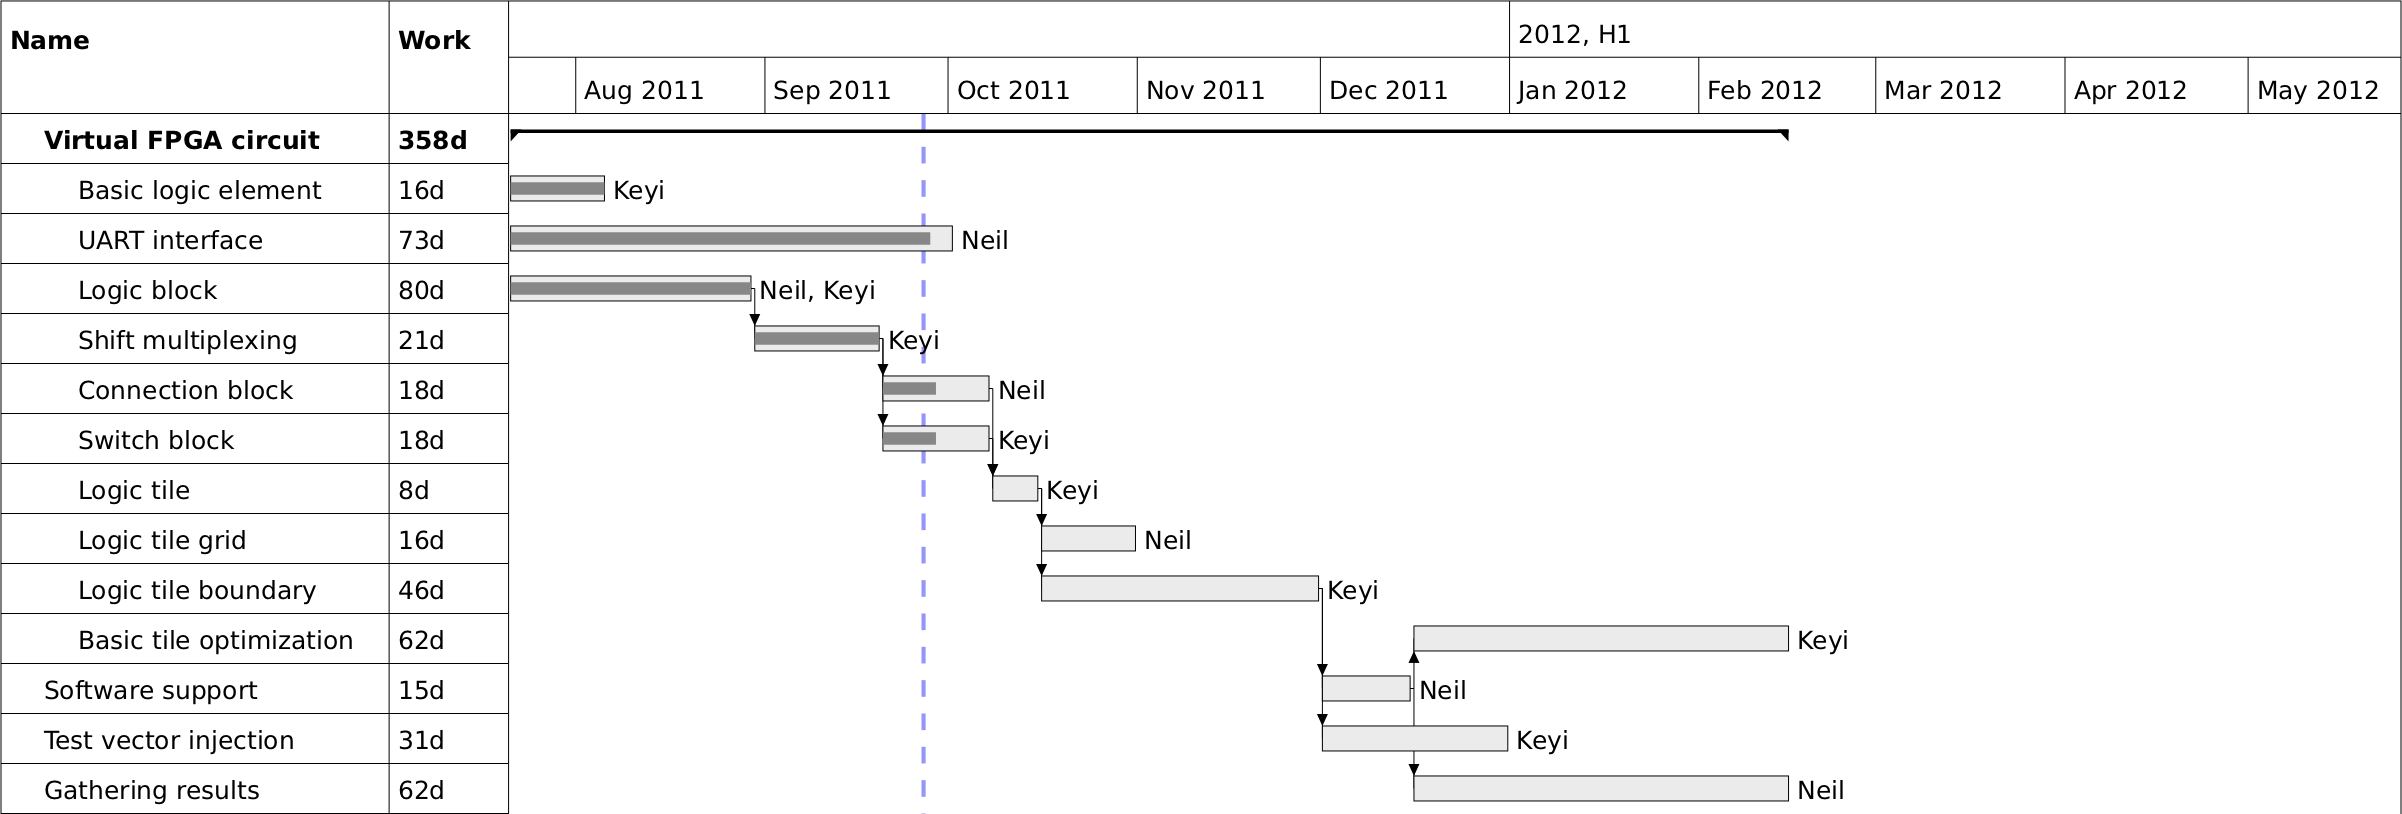
\includegraphics[scale=0.45,angle=90]{gantt.png}


		\section{Validation and Accptance Tests} % from project proposal

\subsection*{Validation and Acceptance Tests from our Project Proposal}

\subsection{Functional validation}

To validate the functional requirements, we will:
\begin{enumeration}
	\item configure the Overlay FGPA and program it onto the physical FPGA,
	\item select and use a benchmark circuit commonly used to test VPR,
	\item configure VPR to match our architecture and dimensions,
	\item place and route the benchmark circuit with VPR,
	\item convert the VPR output into a bitstream for the overlay FPGA,
	\item load the bitstream onto the overlay FPGA, then 
	\item test the functionality of the benchmark circuit running on the overlay FPGA.
\end{enumeration}

The exact verification process for inputs and outputs will depend on the benchmark circuit's intended function.
For the simple test circuits we will test initially, we will set inputs using hardware switches, and observe outputs on LEDs.

Intermediate outputs can also be verified throughout the development process.
We can dump out the bitstream to a text file to verify that it matches the placement and routing in VPR.
We can test the hardware component independently by writing a bitstream by hand as well.


\subsection{Size and overhead validation}

To ensure that the overhead is low enough that the overlay FPGA can fit useful circuits, we will test it using the \emph{``Golden 20''} MCNC benchmark circuits.
For each circuit, we will:
\begin{enumeration}
	\item run synthesis and technology mapping using the ABC synthesis tool,
	\item run placement and routing using VPR configured, and
	\item confirm that VPR can place and route the benchmark circuit using the number and arrangement of logic blocks that we can fit.
\end{enumeration}


	\end{appendices}

	%\pagebreak
	%\fancyhead[L]{Addenda}
	%\addcontentsline{toc}{section}{Title}
	%\section*{Title}
	%\input{file}
	%\pagebreak

\end{document}

